\documentclass[numbers=noenddot, 12pt, a4paper, oneside]{scrbook}
\usepackage{blindtext}
\usepackage[utf8]{inputenc}
\usepackage{float}
\usepackage{tabularx}
\usepackage{graphicx}
\def\Plus{\texttt{+}}
\usepackage{listings}
\usepackage{color}

\definecolor{dkgreen}{rgb}{0,0.6,0}
\definecolor{gray}{rgb}{0.5,0.5,0.5}
\definecolor{mauve}{rgb}{0.58,0,0.82}

\lstset{frame=tb,
	language=Java,
	aboveskip=3mm,
	belowskip=3mm,
	showstringspaces=false,
	columns=flexible,
	basicstyle={\small\ttfamily},
	numbers=none,
	numberstyle=\tiny\color{gray},
	keywordstyle=\color{blue},
	commentstyle=\color{dkgreen},
	stringstyle=\color{mauve},
	breaklines=false,
	breakatwhitespace=true,
	tabsize=3
}


\begin{document}
 
\begin{titlepage}
	\centering
	{\scshape\LARGE Politecnico di Milano \par}
	\vspace{1cm}
	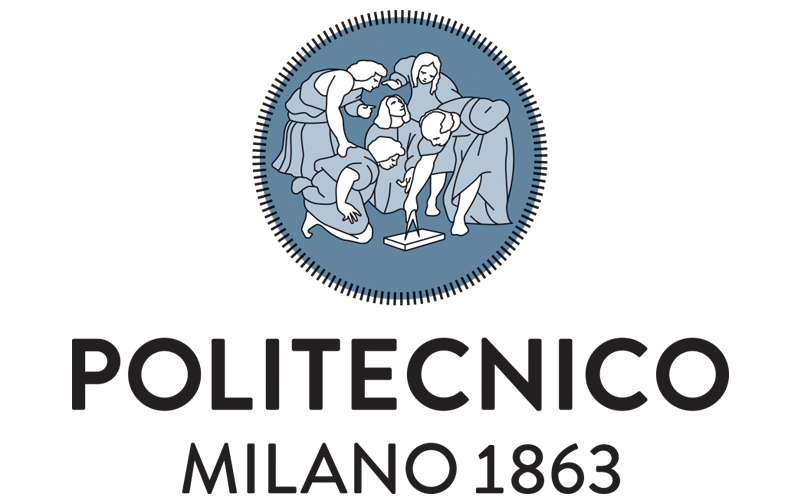
\includegraphics[width=0.35\textwidth]{polimi-logo}\par
	\vspace{1cm}
		
	{\scshape\Large Software Engineering 2 Course\par}
	\vspace{1.5cm}
	{\huge\bfseries Travlendar \Plus \par}
	\vspace{6cm}
	{\Large\itshape di\par}
	{\Large\itshape Gianluigi Oliva, Marco Mussi e Lukasz Moskwa\par}
	\vfill

	
	\vfill
	
	% Bottom of the page
	{\large \today\par}
\end{titlepage}

\newpage 
\tableofcontents
\newpage 

\section*{Abstract}


\chapter{Introduction}



\section{Purpose}

The purpose of this document is to provide technical details about the information contained in
RASD of Travelandar+ Application and lead the developers that viewing this document can develop the application in the correct way.\\

The output of this document is an architectural description that shows all the critical feature of the
problem taken into account.
In particular in this document will be treated:
\begin{itemize}
	\item The high architectural level;
	\item The design patterns;
	\item The main component and the interface that the application provides;
	\item The runtime behavior;
	\item The data structure used for the developing;
\end{itemize}

The relation among the different models is represented by using UML diagram and other useful
kind of diagram that show the structure of the system (Entity – Relation diagram).



\section{Scope}

The scope of this application (Travlendar \Plus) is provide a tool for the target users to schedule in an effective way their time optimizing the travels.\\

Travlendar+ allows to create a calendar which fits the meetings and other kind of commitments.
The key feature of this application is to determine if the meeting location is reachable in the scheduled time and then provide a fast way to get to the destionation, otherwise it notify the user that it is not possibile by any mean to fullfill the request. Furthermore the application also arranges the schedule in a flexible way, taking into account weather condition and user's preferences as well, for some kind of events (like the lunch) and offers the possibility to slightly change its time.\\

With Travlendar+ is possible as well to buy public transport's tickets on the fly for the journey. If the user requires often the same path, he is suggested by the application to buy the best offered subscription.\\

The architecture must be designed with the intent of being maintainable and extensible. For this purpose, we will implement some known design patterns which will facilitate the development of the system.



\section{Definitions, Acronyms, Abbreviations}

\subsection*{Definitions}
\begin{itemize}
	\item \textbf{Platform}: system/application as a whole.
	\item \textbf{User}: An end user who is currently registered to the Travlendar+ application and has credentials to access.
	\item \textbf{Guest}: Person not registered yet and with limited access to features.
	\item \textbf{Event}: A scheduled meeting or other kind of appointment a user has to attend.
	\item \textbf{Journey}: The path chosen by the application as the one with all the fullfilled requirements.
	\item \textbf{Bad Weather}: A weather that prevents the user from choosing some path options. The listed bad weathers are snow, rain, storm and others.
	\item \textbf{Framework}: Reusable set of libraries or classes for a software system.
	\item \textbf{Cross-Platform}: software able to run on different platforms with same code.
	\item \textbf{Port}: in the internet protocol suite, it is an endpoint of communication in operating system
	\item \textbf{Web-Socket}:is a computer communications protocol, providing full-duplex communication channels over a single TCP connection
	\item \textbf{REST}: is a way of providing interoperability between computer systems on the Internet.
	\item \textbf{RESTful}: a system using REST
	\item \textbf{Client Server Architecture}:  is a distributed application structure that partitions tasks or workloads between the providers of a resource or service, called servers, and service requesters, called clients.
	\item \textbf{Client Tier}: is the tier/layer involving the client.
	\item \textbf{Fat Client}: is a client computer in client–server architecture or networks that typically provides rich functionality independent of the central server.
	\item \textbf{Layer}:In a logical multilayered architecture for an information system with an object-oriented design, the main layers are Presentation layer, Application layer and Data access layer.
\end{itemize}

\subsection*{Acronyms}

\begin{itemize}
	\item \textbf{RASD}: Requirements Analysis and Specification Document
	\item \textbf{DB}: Database
	\item \textbf{DBMS}: Database Management System
	\item \textbf{OS}: Operating System 
	\item \textbf{HTML}: HyperText Markup Language
	\item \textbf{CSS}: Cascading Style Sheets
	\item \textbf{JS}: JavaScript
	\item \textbf{JSON}: JavaScript Object Notation
	\item \textbf{API}: Application Programming Interface
	\item \textbf{IDE}: Integrated Development Environment
	\item \textbf{RAM}: Random Access Memory
	\item \textbf{HTTP}: HyperText Transfer Protocol
	\item \textbf{HTTPS}: HyperText Transfer Protocol Secure
	\item \textbf{TCP}: Transmission Control Protocol
	\item \textbf{ACID}: Atomicity Consistency Isolation and Durability
	\item \textbf{DD}: Design Document
	\item \textbf{MVC}: Model View Component
	\item \textbf{UX}: User Experience
	\item \textbf{URL}: Uniform Resource Locator
	\item \textbf{OLTP}: On Line Transaction Processing
	
\end{itemize}

\subsection*{Abbreviations}
\begin{itemize}
	\item \textbf{Gn}: n-th goal
	\item \textbf{Rn}: n-th functional requirement
	\item \textbf{Dn}: n-th domain
	\item \textbf{Mn}: n-th mockup
	\item \textbf{WebApp}: WebApplication 
\end{itemize}



\section{Revision History}

Version, date and summary\\

\begin{tabular}{|p{0.2\textwidth}|p{0.3\textwidth}|p{0.4\textwidth}|}
	\hline
	\parbox[c][6ex]{6ex}{\centering \textbf{Version}} & \textbf{Date} & \textbf{Summary}\\
	\hline
	\parbox[c][6ex]{6ex}{\centering 1.0.0} & \today & First release of this document\\
	%	\parbox[c][6ex]{6ex}{\centering \textbf{Goal}} & 2 \\
	\hline
	
	
	
\end{tabular}



\section{Reference Documents}


We used the following documents:
\begin{enumerate}
	\item The orginal Travlendar application: \\
	\textbf{http://score-contest.org/2018/projects/travlendar.php}
	\item The revised document of the assignment:\\
	\textbf{https://goo.gl/9m1ojy}
	
	\item IEEE Std 830-1998 IEEE Recommended Practice for Software Requirements Specifications. 
	
	\item IEEE Std 1016tm-2009 Standard for Information Tecnology-System Design-Software Design Descriptions.
\end{enumerate}

\section{Document Structure}


\begin{itemize}
	\item \textbf{Introduction}: This section provides a general introduction and overview of the Design Document
	\item \textbf{Architectural Design}: Overall description of the main system component and relationship between them. This part is divided in various subsection in which are show the main component view, deployment view, runtime view, component interface and design patterns.
	\item \textbf{Algorithm Design}: Overall description of the high level details about the most critical part of the algorithms that must be implemented for the system.
	\item \textbf{User Interface Design}: Overview of the way the user can interact with the system and the response of the application to the user input.
	\item \textbf{Requirements Traceability}: Overview of how the design part descripted in this document
	satisfy the functional requirement and the constraints explain the RASD.
	\item \textbf{Implementation, Integration and Test Plan}: Identification of the order we will use to realize the subcomponents of the system and how we will integrate and test them together.
	\item \textbf{Effort Spent}: Time and resource effort during the development of the application.
	\item \textbf{References}: References and software used during the process of creation of the system.
\end{itemize}




\chapter{Architectural Design}

\section{Overview: Highlevel components	and their interaction}

The Travlander+ system has a three tier architecture:

\begin{figure}[H]
	\centering
	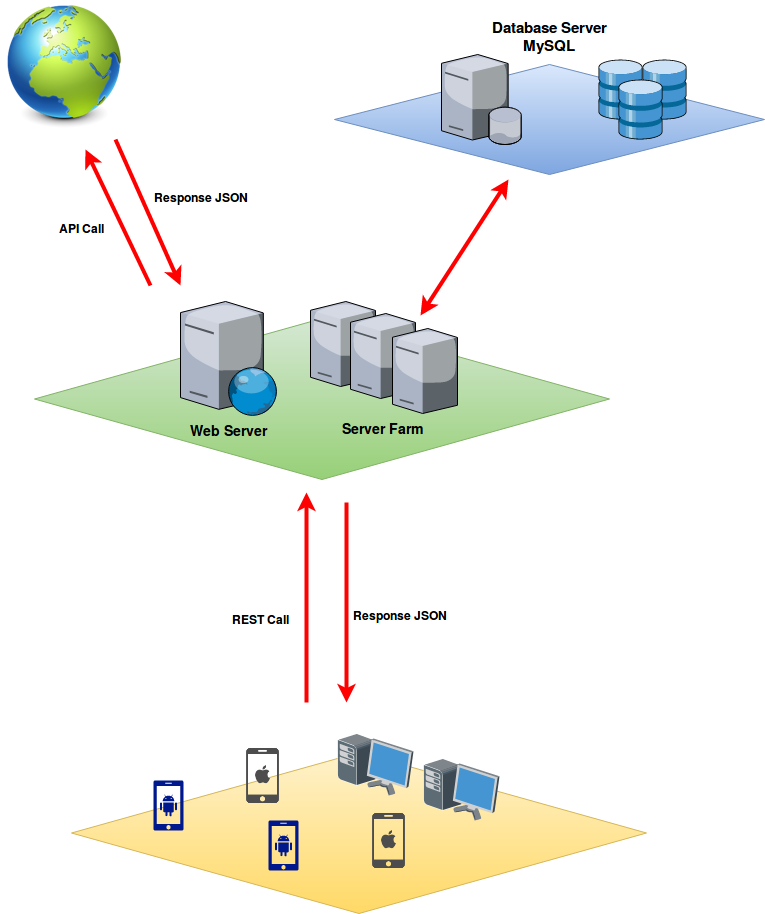
\includegraphics[width=0.7\textwidth]{images/HighLevelArchitecture}
	\caption{Graphical description of the High Level Architecture and relationship of the tiers}
\end{figure}

The client has only the presentation layer realized with a dynamic GUI, created due to informations retrieved by the server. The communication between client and server happens due to REST calls and JSON response.\\

The second tier contains the application logic layer and the methods for the communication with the Database Server.\\

The third layer stores all the usefull data to the user which allows the system to perform operations and manage separatly different users.

\begin{figure}[H]
	\centering
	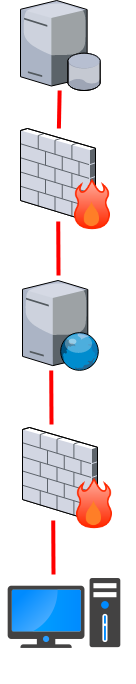
\includegraphics[width=0.2\textwidth]{images/ArchitectureLayer}
	\caption{Graphical representation of the position of the firewalls in our network}
\end{figure}

Between all the layers there are firewalls in order to increase the safety of communication and increase the reliability of the overall system.

\subsection*{High level component}

The high level components architecture is composed of four different elements
types. The main element is a singleton, the web server.
Clients communicate only with the web application server and this kind of communication can be performed throught a PC, a mobile device and all devices which allow the execution of JavaScript.\\

When the client has to perform a request, it sends a well formatted JSON string to the web application that will computate it, interacting as well with third part services and with the database if needed to save or to request usefull information, and provide a response.\\

The client and the server communicate using both synchronous messages and asynchronous ones based on the purpose. For example, if the user wants to save some informations, a synchronous communication will be done. Otherwise if, for example, a client requires the informations of a map (that is retrieved with the Google's API) an asynchronous communication will be done.\\

\begin{figure}[H]
	\centering
	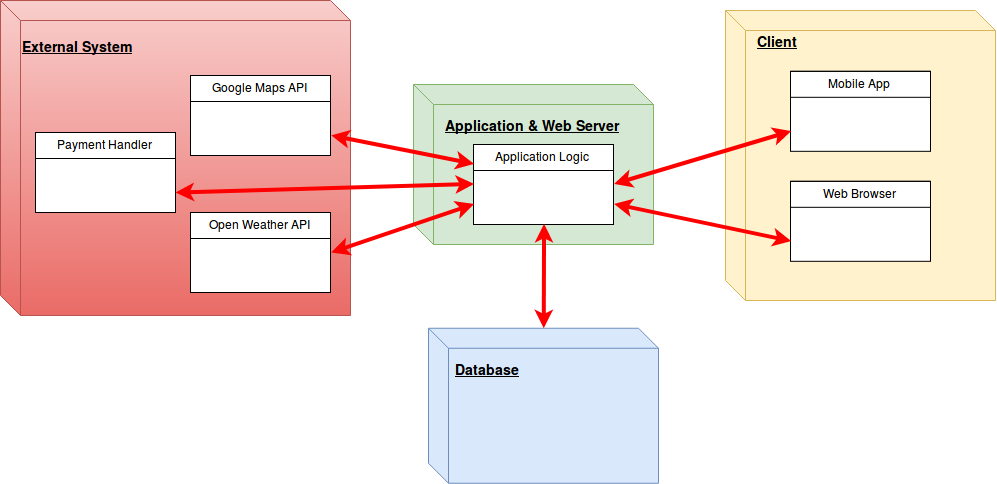
\includegraphics[width=1.1\textwidth]{images/HighLevelComponent}
	\caption{Graphical representation of the High Level components}
\end{figure}

\section{Component View}

In this section we will explain in detail all the major sub-part of the system and the way they interact each other.

\subsection*{DBMS Server}

Into the database server we want to use a relational DBMS component, like MySQL, to manage the interaction with the database. In that way we can guarantee the ACID properties of the transactions executed.\\

As seen in the previous schema (Fig 2.2) the DBMS server can communicate only with the Application server through a firewall. Sensible data such as passwords and personal information must be encrypted properly before being stored. Users must be granted access only upon provision of correct and valid credentials.\\

The DBMS will use a high level schema like the one represented in the following Entity-Relationship diagram.\\

The main components of the DBMS server are:
\begin{itemize}
	\item \textbf{DBMS}:\\\newline
	This component deals with the operations of read and write of the data stored into the Database. It's implemented as OLTP, which is used to refer to processing in which the system responds immediately to user requests.\\
	
	\item \textbf{DBRequestHandler}:\\\newline
	This module converts requests from the Application Server into SQL queries which are executed by the DBMS.\\
	
\end{itemize}



\begin{figure}[H]
	\centering
	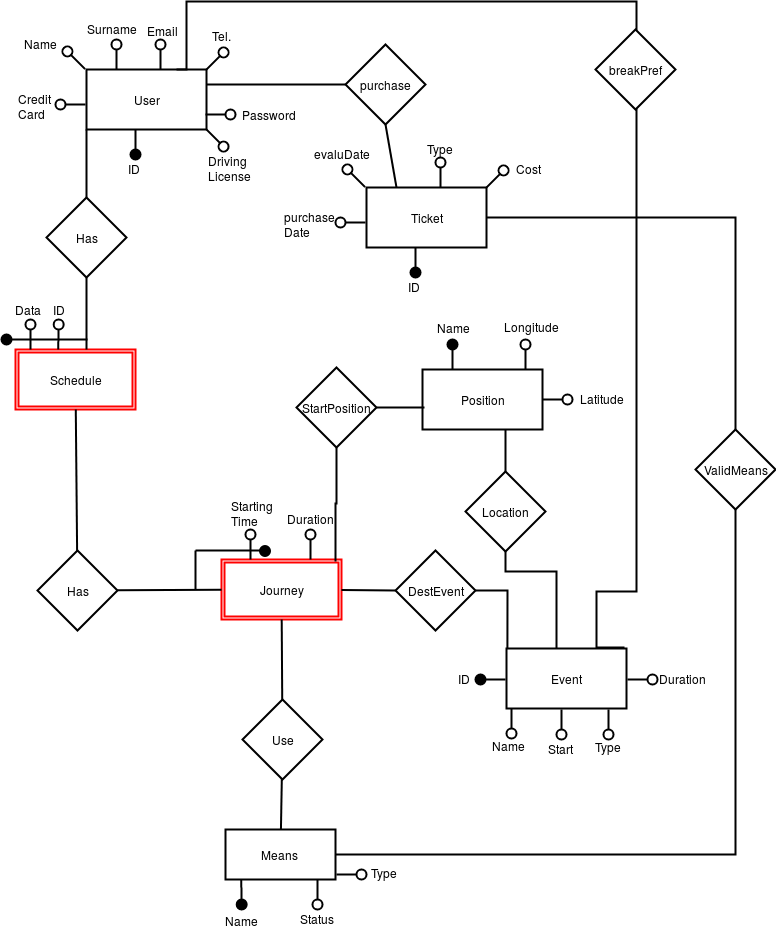
\includegraphics[width=1.1\textwidth]{images/ER}
	\caption{E-R Diagram of the DBMS}
\end{figure}


\subsection*{Application and Web Server}

For our purpose we decided to merge together the Application and Web server. This choice is based on the three-tier architecture model. The Application server is the middle-tier which implements the business logic of the WebApp. It also uses a Script Engine mechanism to provide dynamic real-time contents to the users.\\

In this layer we can also find a Web Server which is the component that handles the requests from the clients. These requests are based both on HTTP standard protocol and on the Web-Socket protocol. Once the page request is completed, a connection is estabilished with the Web-Socket protocol in order to have a full-duplex communication and refresh the web page content without reloading the whole page.\\

The system must also provide a way to communicate with external systems with the purpose of collecting important data and informations which will allow the correct execution of operations.\\

The main components are:
\begin{itemize}
	\item \textbf{UserManager}:\\\newline
	This module will manage all the sensitive informations about the users. It will also allow the users to see and modify them when requested. It mananages as well the Login and Registration procedures.\\
	
	\item \textbf{ScheduleManager}:\\\newline
	This module contains the business and application logic that performs the computation of the best travel path and also verifies the schedule can fit in the user's timetable. In order to provide the best journey path, this module takes into account the weather forecast as well through the ExternalRequestManager.\\
	
	\item \textbf{ExternalRequestManager}:\\\newline
	This module handles all the communications with third part services and retrives from them important informations which will be passed to other system's modules. \\
	
	\item \textbf{PaymentHandler}:\\\newline
	This module deals with all the procedures necessary to perform a payment. This occurs every time a user wants to purchase a ticket or a subscription for a specific journey in his schedule. In some cases, with third part services like car sharing or bike sharing, this module redirects those informations directly to the required service page.\\
	
	\item \textbf{SecurityAuthenticator}:\\\newline
	This module manages all the security policies in order to prevent fraudulent accesses and guarantee the privacy of the users. It also provide a secure way to connect to the web application using a token-based mechanism in a Web-Socket context. \\
	
	\item \textbf{NotificationManager}:\\\newline
	The Notification Manager purpose is to handle all the notifications to the user and communicate them even when the application is closed or in background. It also report the informations on different priority levels.\\
	
	\item \textbf{RequestController}:\\\newline
	This module has the task of managing all the user's requests and handle them to the proper system modules in order to fullfill their queries.\\
	
	\item \textbf{DataHandler}:\\\newline
	This module allows the exchange of data and informations between the Application/WebServer and the Database Server. While the communication between the Client and the Web Application is made through a HTTPS standard protocol to ensure the connection safety, the communication between the Application Server and the Database is realized with HTTP. In fact, the firewall is configured to deny all the possible connections coming from sources different than the WebApp.\\
	
\end{itemize}

\subsection*{Client}

The client in our model architecture is a Thin Client, as the whole business logic and calculations are made on the Application Server side. Therefore the client realizes only the Presentation Layer.\\

The Client side is meant for the mobile and desktop users and, in order to access to all the system features, it has to have implemented necessary methods to retrieve informations from its GPS hardware component.\\

The client's main components are:

\begin{itemize}	
	
	\item \textbf{PositionController}:\\\newline
	This module takes into account the position of the used device when the ApplicationController needs it. The user is asked either to insert manually his position or grant to the device the permission of using GPS position data.\\
	
	\item \textbf{UIManager}:\\\newline
	This module is used to manage all the contents displayed to the user in a certain page he visits. It takes datas from the ApplicationController and show them. It is also responsible for the handling of user's input and form fullfilling.\\
	
	\item \textbf{NotificationMonitor}:\\\newline
	This software component has the purpose of listen the Application server notifications and display them immediatly or, if expected, store them for a while and then display them when scheduled.\\
	
	\item \textbf{ApplicationController}:\\\newline
	This module acts as core of our client implementation. It contains the client's logic and allows an efficent communication between modules listed above.\\
	
	This software component deals with all the user's request and forward them through a specific protocol in a public network to the Application Server.
	It also handles the retrived data received as responses from the Server side, and send them to the ApplicationController to be shown.\\
	
\end{itemize}


\begin{figure}[H]
	\centering
	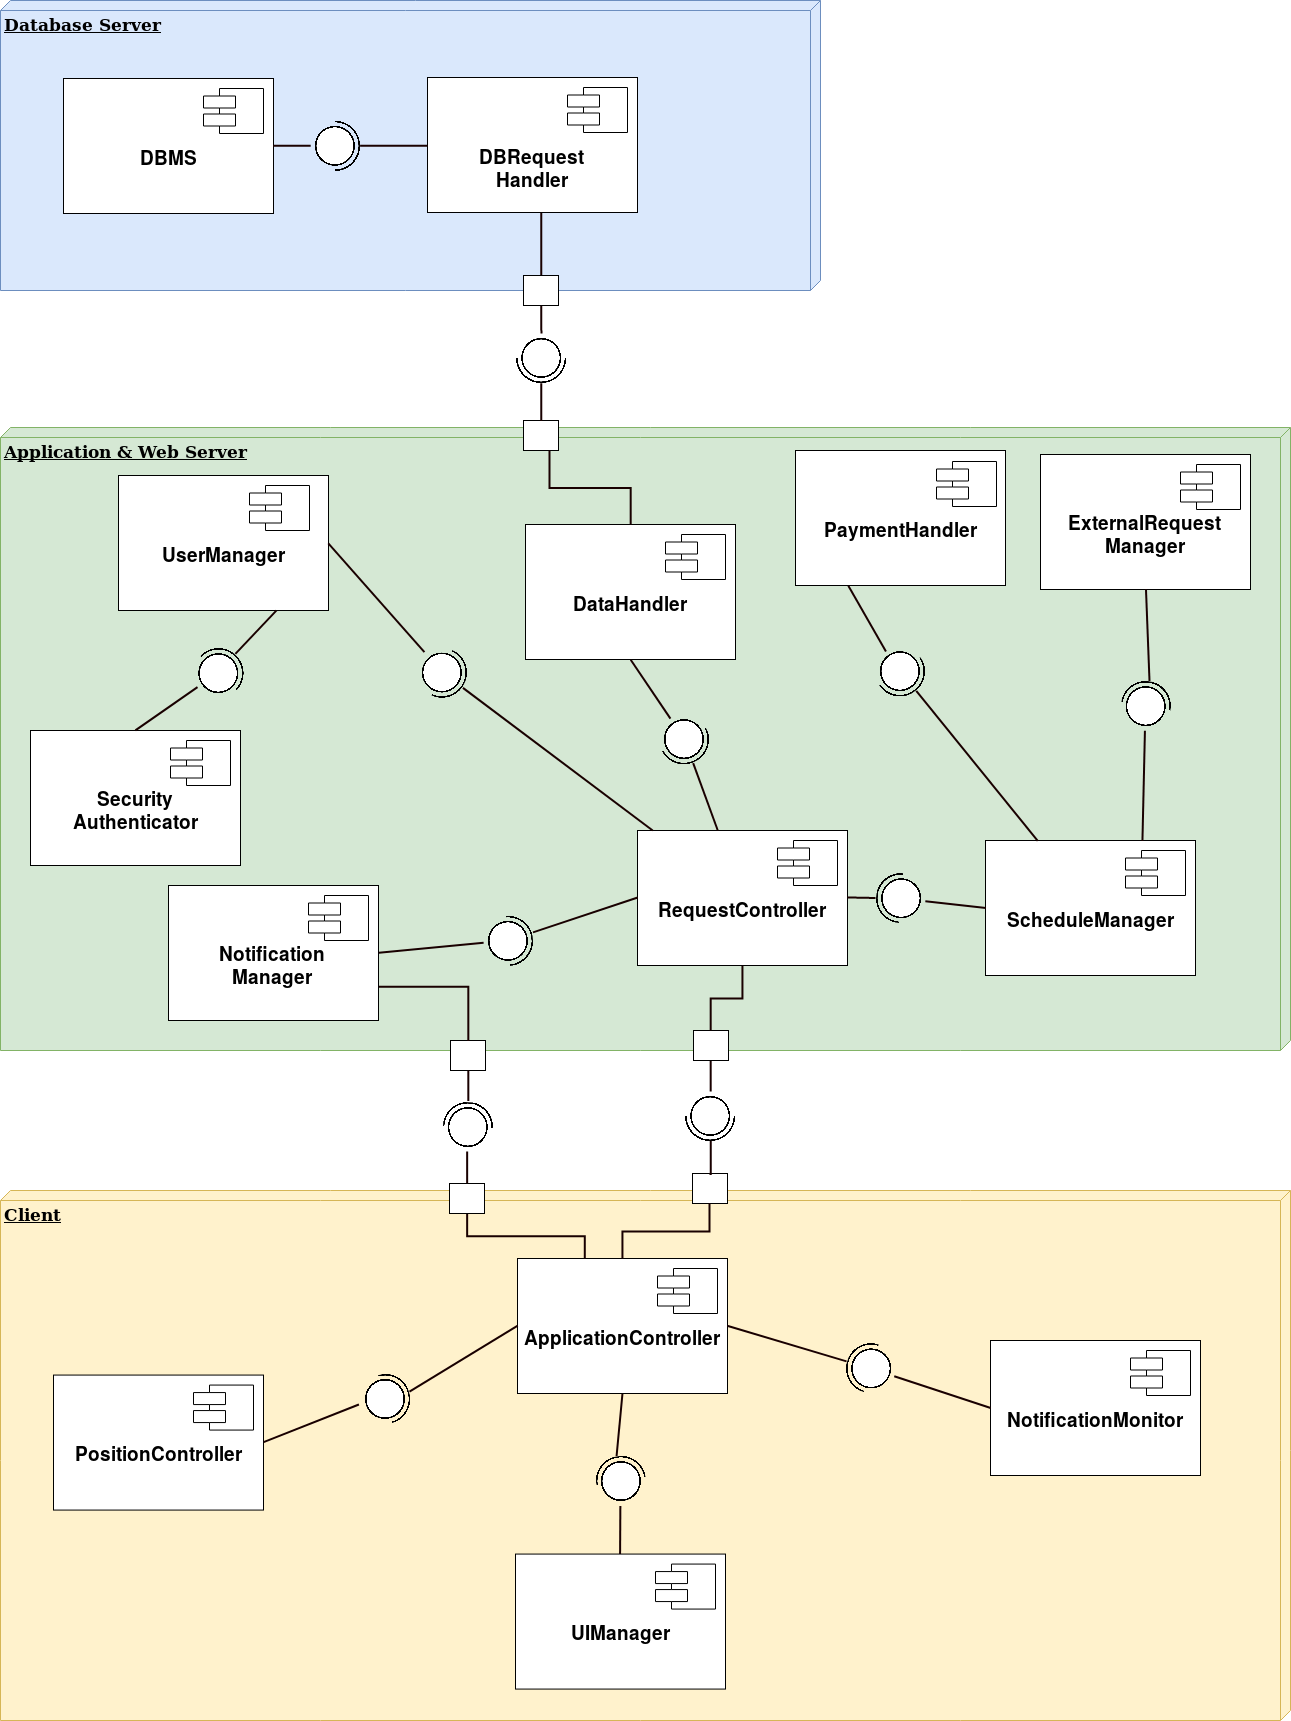
\includegraphics[width=0.95\textwidth]{images/ComponentView}
	\caption{Component View of the System}
\end{figure}


\section{Deployment View}


\begin{figure}[H]
	\centering
	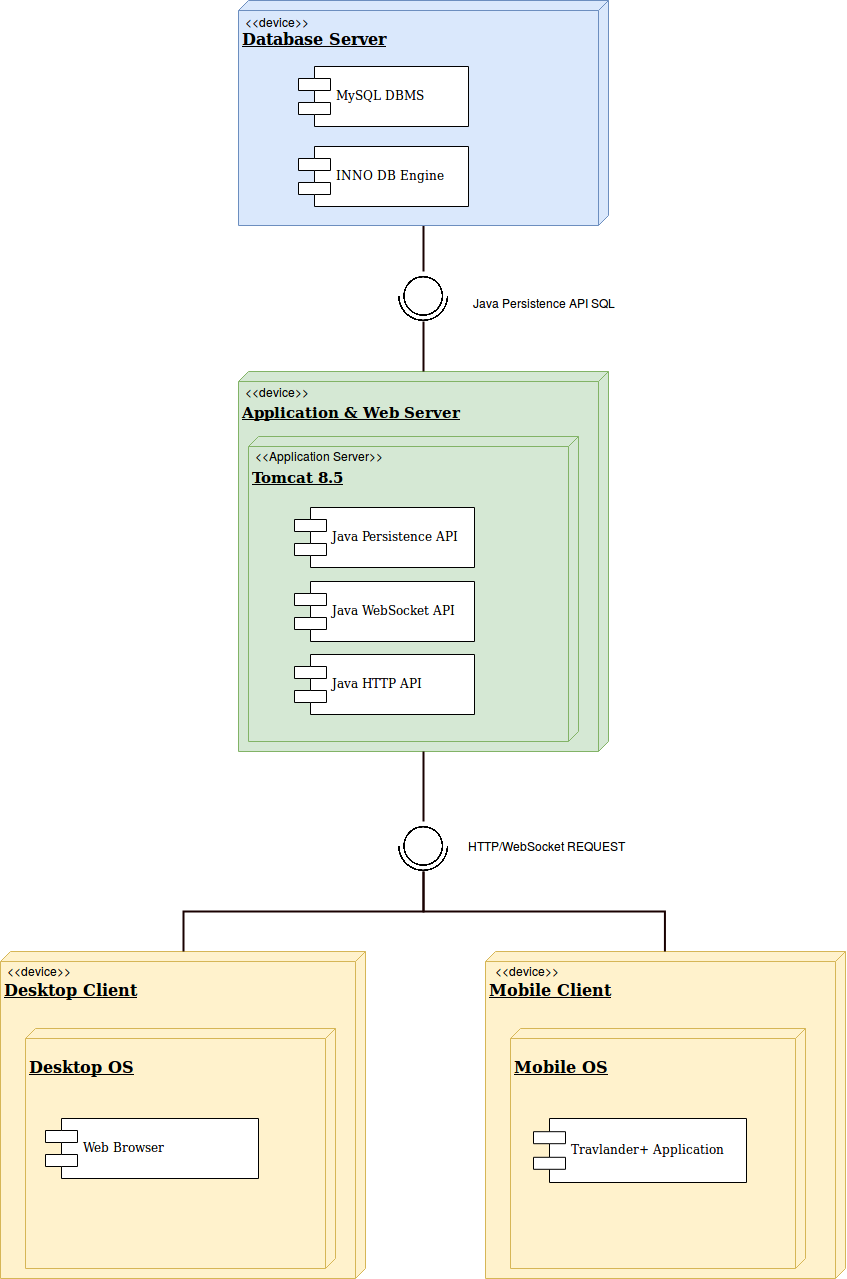
\includegraphics[width=0.80\textwidth]{images/DeploymentView}
	\caption{Deployment View of the system}
\end{figure}


\section{Runtime View}

This section represents the dynamic behaviour of the system in the most
relevant and already seen cases. The purpose of each of the following sequence diagrams is to explain as much as possibile in the detail, the workflow inside the Application Server and its communication with the Client and the Database Server.

\subsection*{Registration to Travlendar+ application}

\begin{figure}[H]
	\centering
	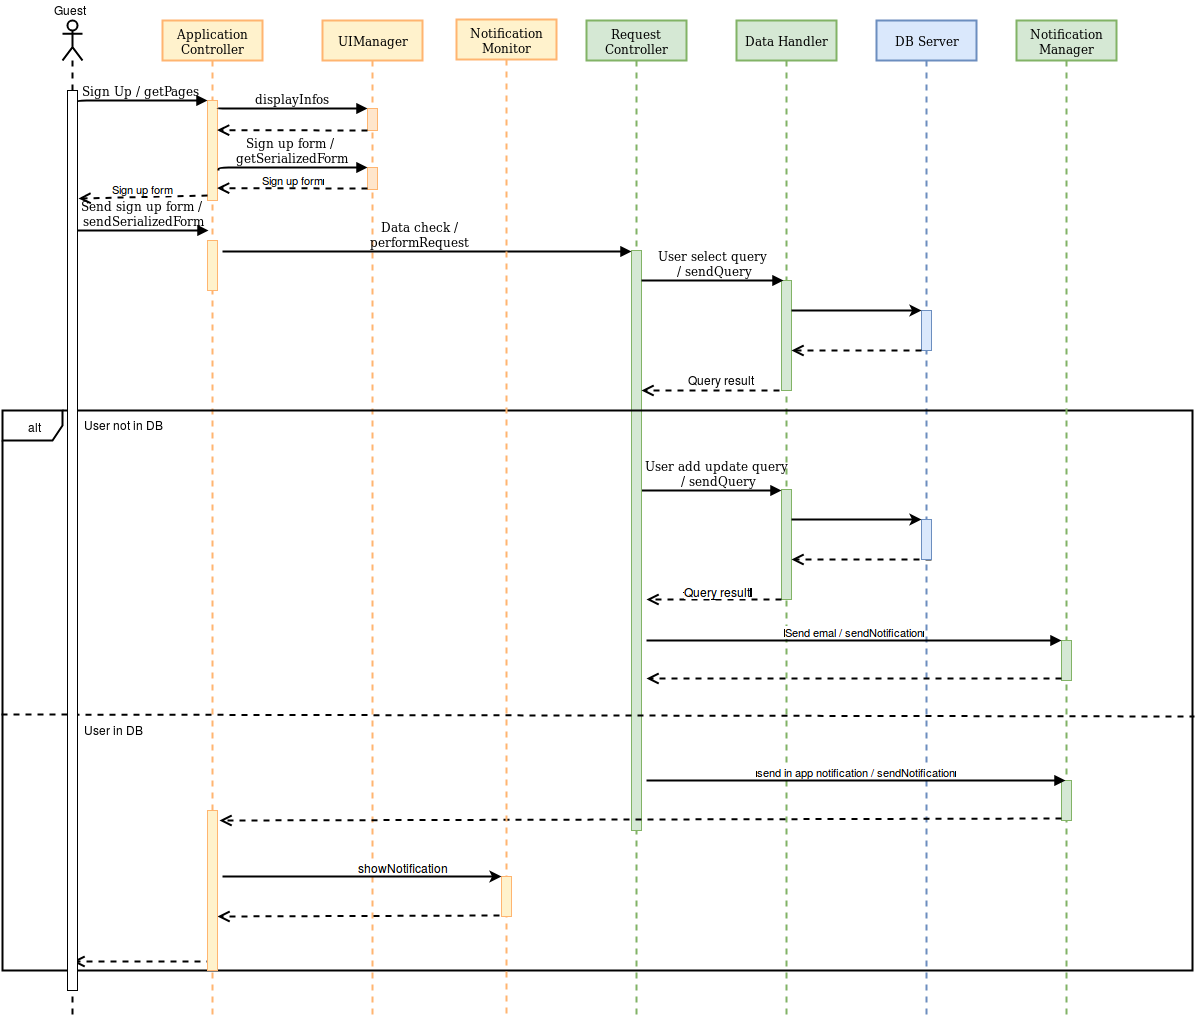
\includegraphics[width=1.1\textwidth,angle=-0]{images/Goal1}
	\caption{Sequence Diagram of the guest's registration to the application}
\end{figure}

As we can see in this Diagram, the guest can send a Serialized Form from the Application Controller module to the Request Controller, which will entrust the Data Handler of making a request to the Database Sever in order to know if a user with same datas already exists.\\

If not, the guest is added to the Database server and is sent an e-mail for account verification. Otherwise, the guest is notified that someone with the same datas already exists.

\subsection*{Schedule Creation}

\begin{figure}[H]
	\centering
	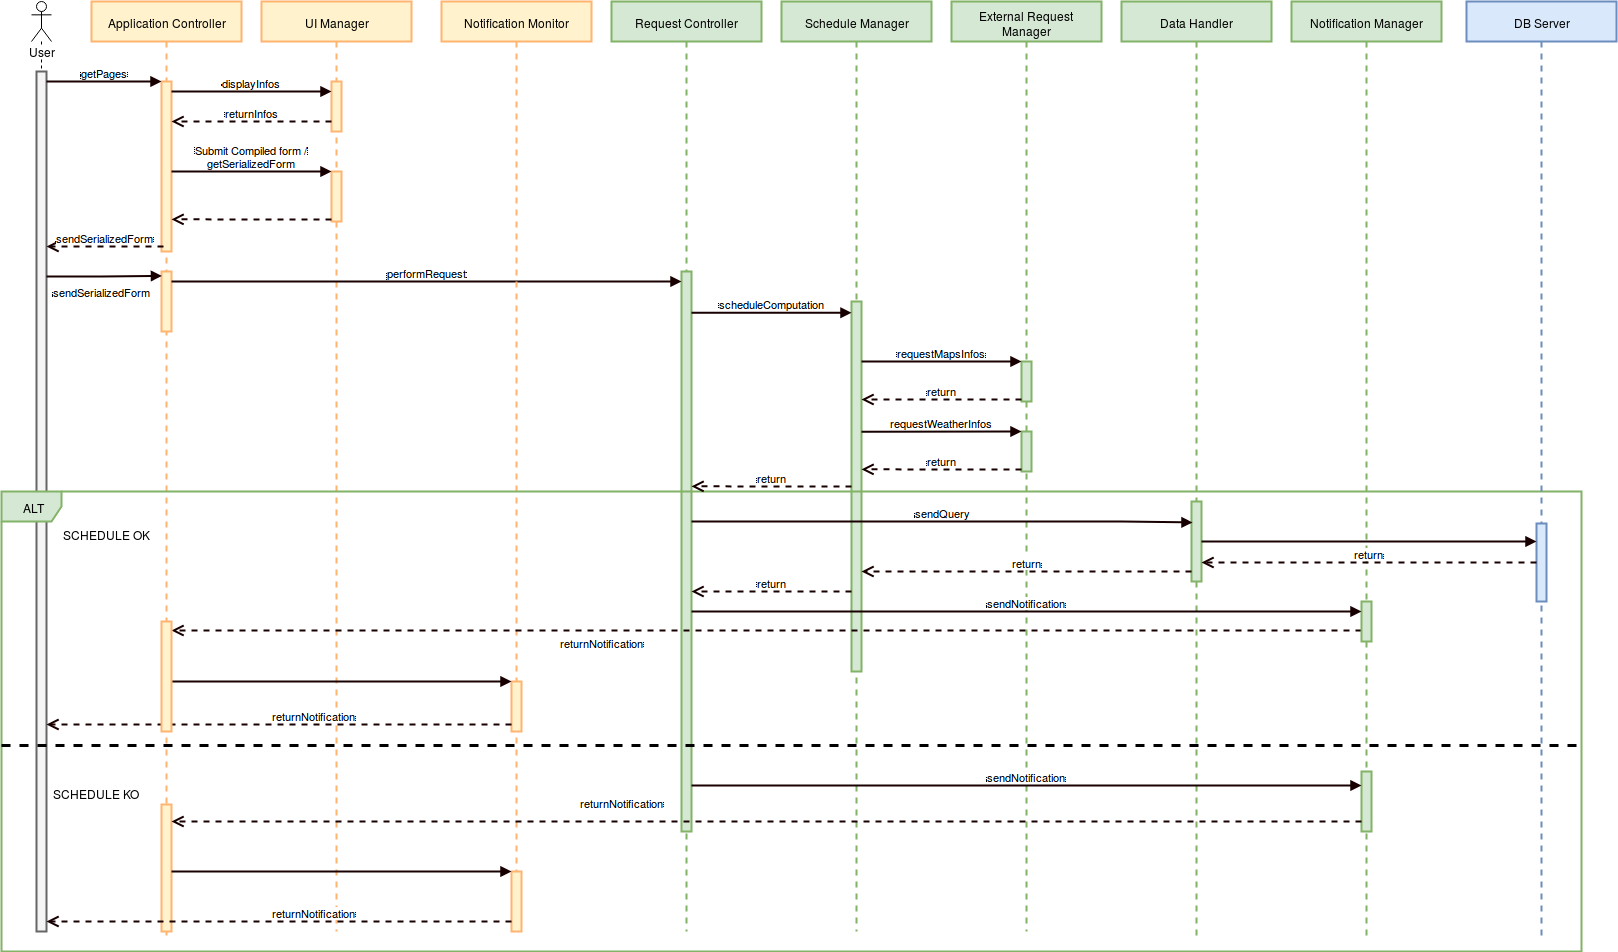
\includegraphics[width=1.1\textwidth,angle=-0]{images/Goal2}
	\caption{Sequence Diagram of the schedule creation}
\end{figure}

In this diagram is possible to see how the components interact between them in order to create a new schedule. Once the request reaches the Application server, several control are made and the External Request Manager grants informations about the Weather and path to be chosen.


\subsection*{Manage User's information}

\begin{figure}[H]
	\centering
	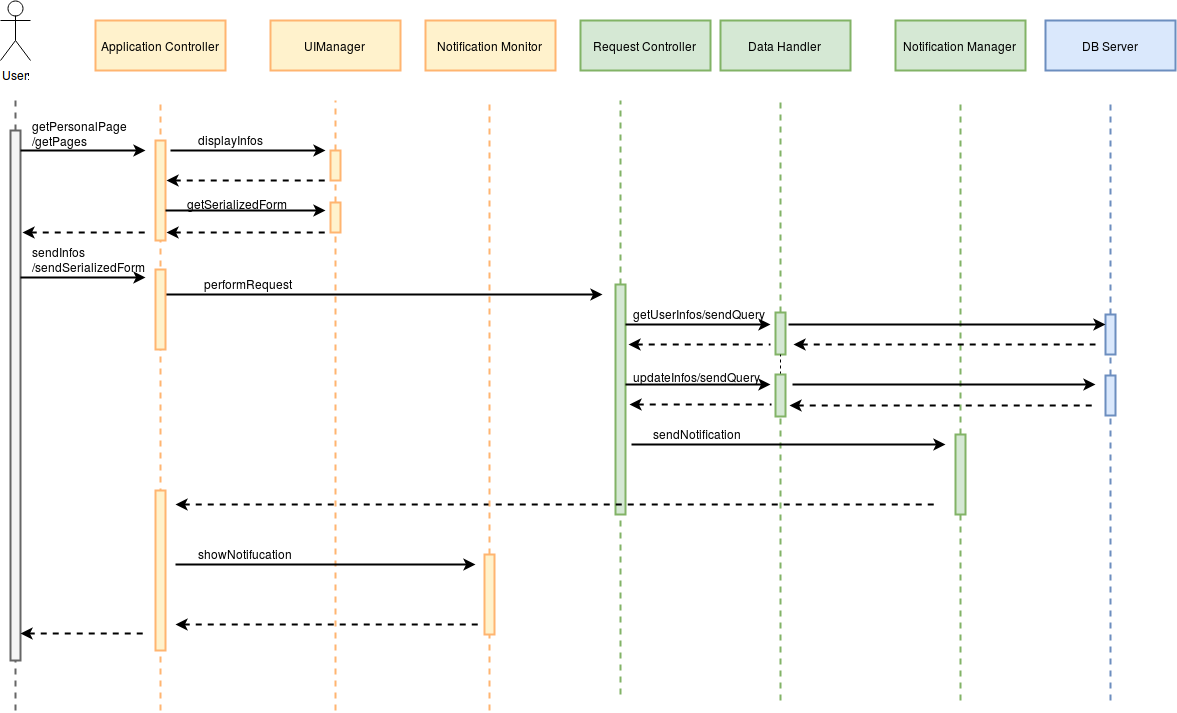
\includegraphics[width=1.1\textwidth,angle=-0]{images/Goal3}
	\caption{Sequence Diagram of the managing of users' information}
\end{figure}

In this diagram it is possible to see how the Data Handler module deals with a request of the user to modify his data and preferences. All the changes are stored in the DB Server.


\subsection*{Retrieve Weather Forecast informations}

\begin{figure}[H]
	\centering
	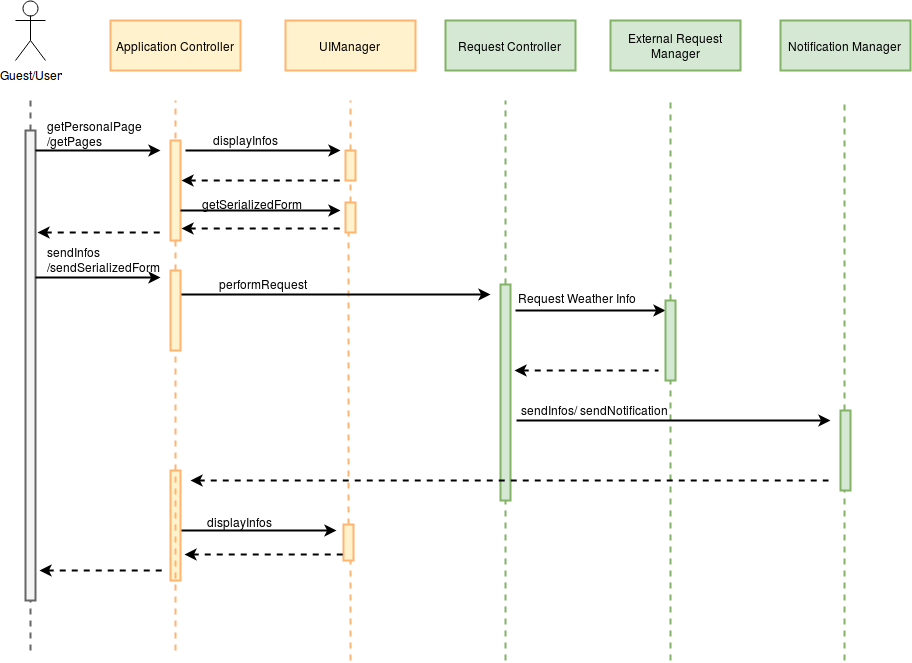
\includegraphics[width=1.1\textwidth,angle=-0]{images/Goal4}
	\caption{Sequence Diagram of the retrieving of Weather Forecast informations}
\end{figure}

Both the guests and users can actually retrieve informations about the Weather Forecast. This is done by the External Request Manager that collect datas from the Openweather external API. Then these informations are sent to the Notification Manager module.

\subsection*{Buy tickets and subscription for public transport}

\begin{figure}[H]
	\centering
	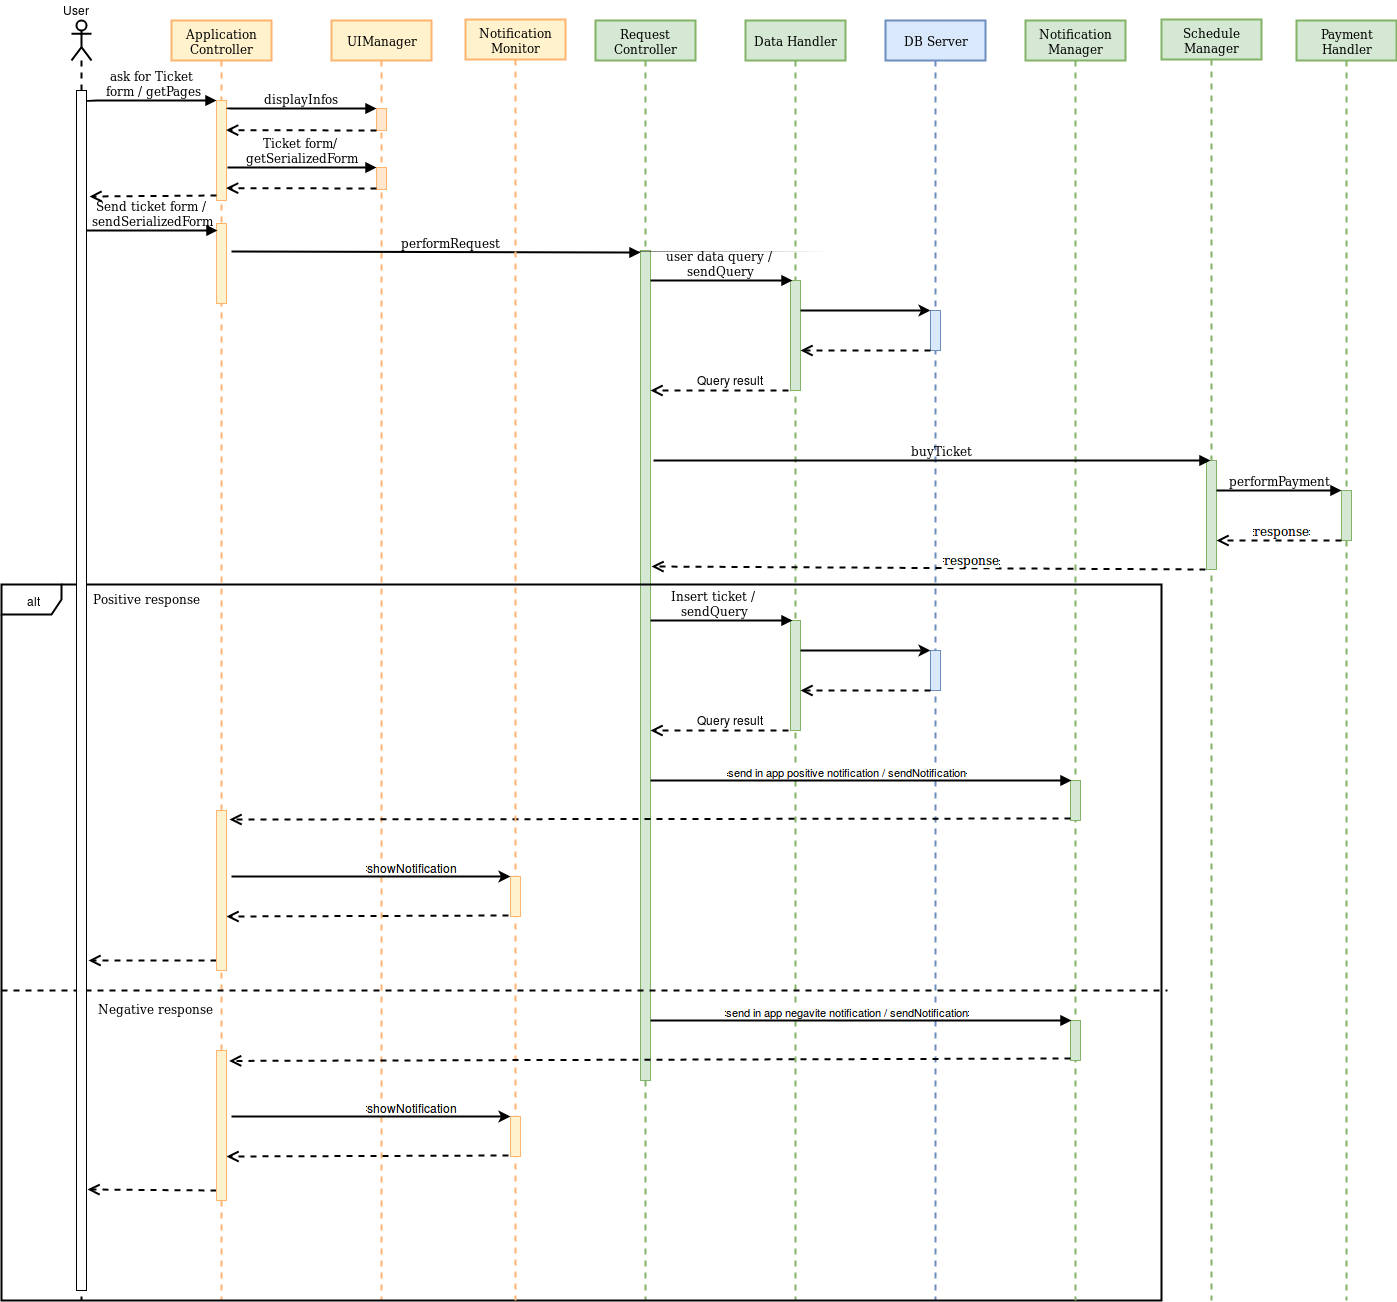
\includegraphics[width=1.1\textwidth,angle=-0]{images/Goal5}
	\caption{Sequence Diagram of the purchase of tickets and subscription for public transport}
\end{figure}

Here we can observe the procedure that deals with the purchase of tickets by the user. If the transaction done due to the Payment Handler goes well, the informations about the bought ticket are saved to the Database Server using the submitQuery method.

\subsection*{Share user's schedule}

\begin{figure}[H]
	\centering
	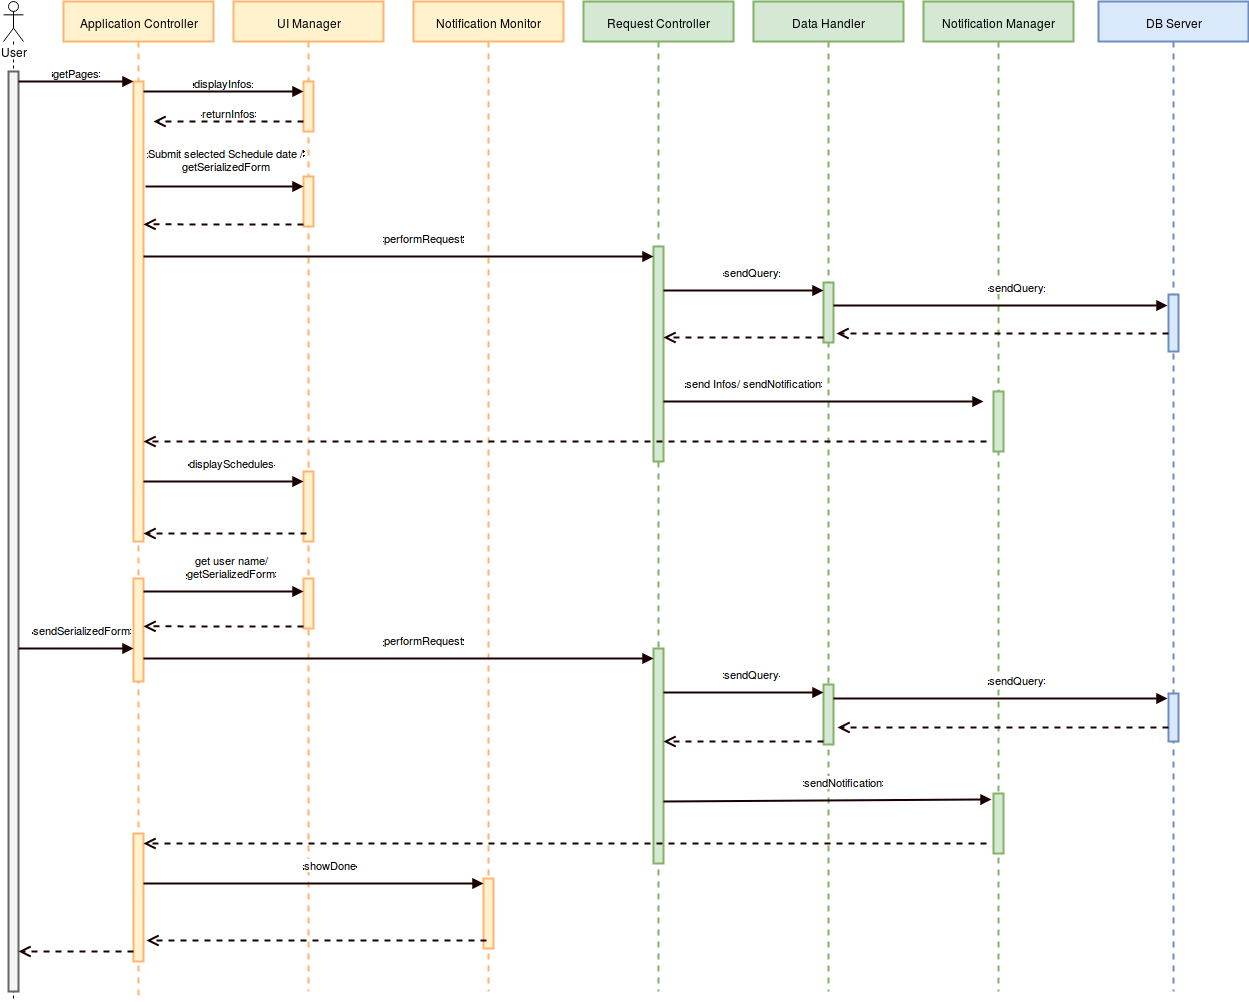
\includegraphics[width=1.1\textwidth,angle=-0]{images/Goal6}
	\caption{Sequence Diagram of sharing user's schedule}
\end{figure}

Whenever a user wants to share his own schedule of a given day of his choice, the username of the second user is saved to the Database Server. Then the first user is notified by the Notification Manager.

\subsection*{Update user's schedule}

\begin{figure}[H]
	\centering
	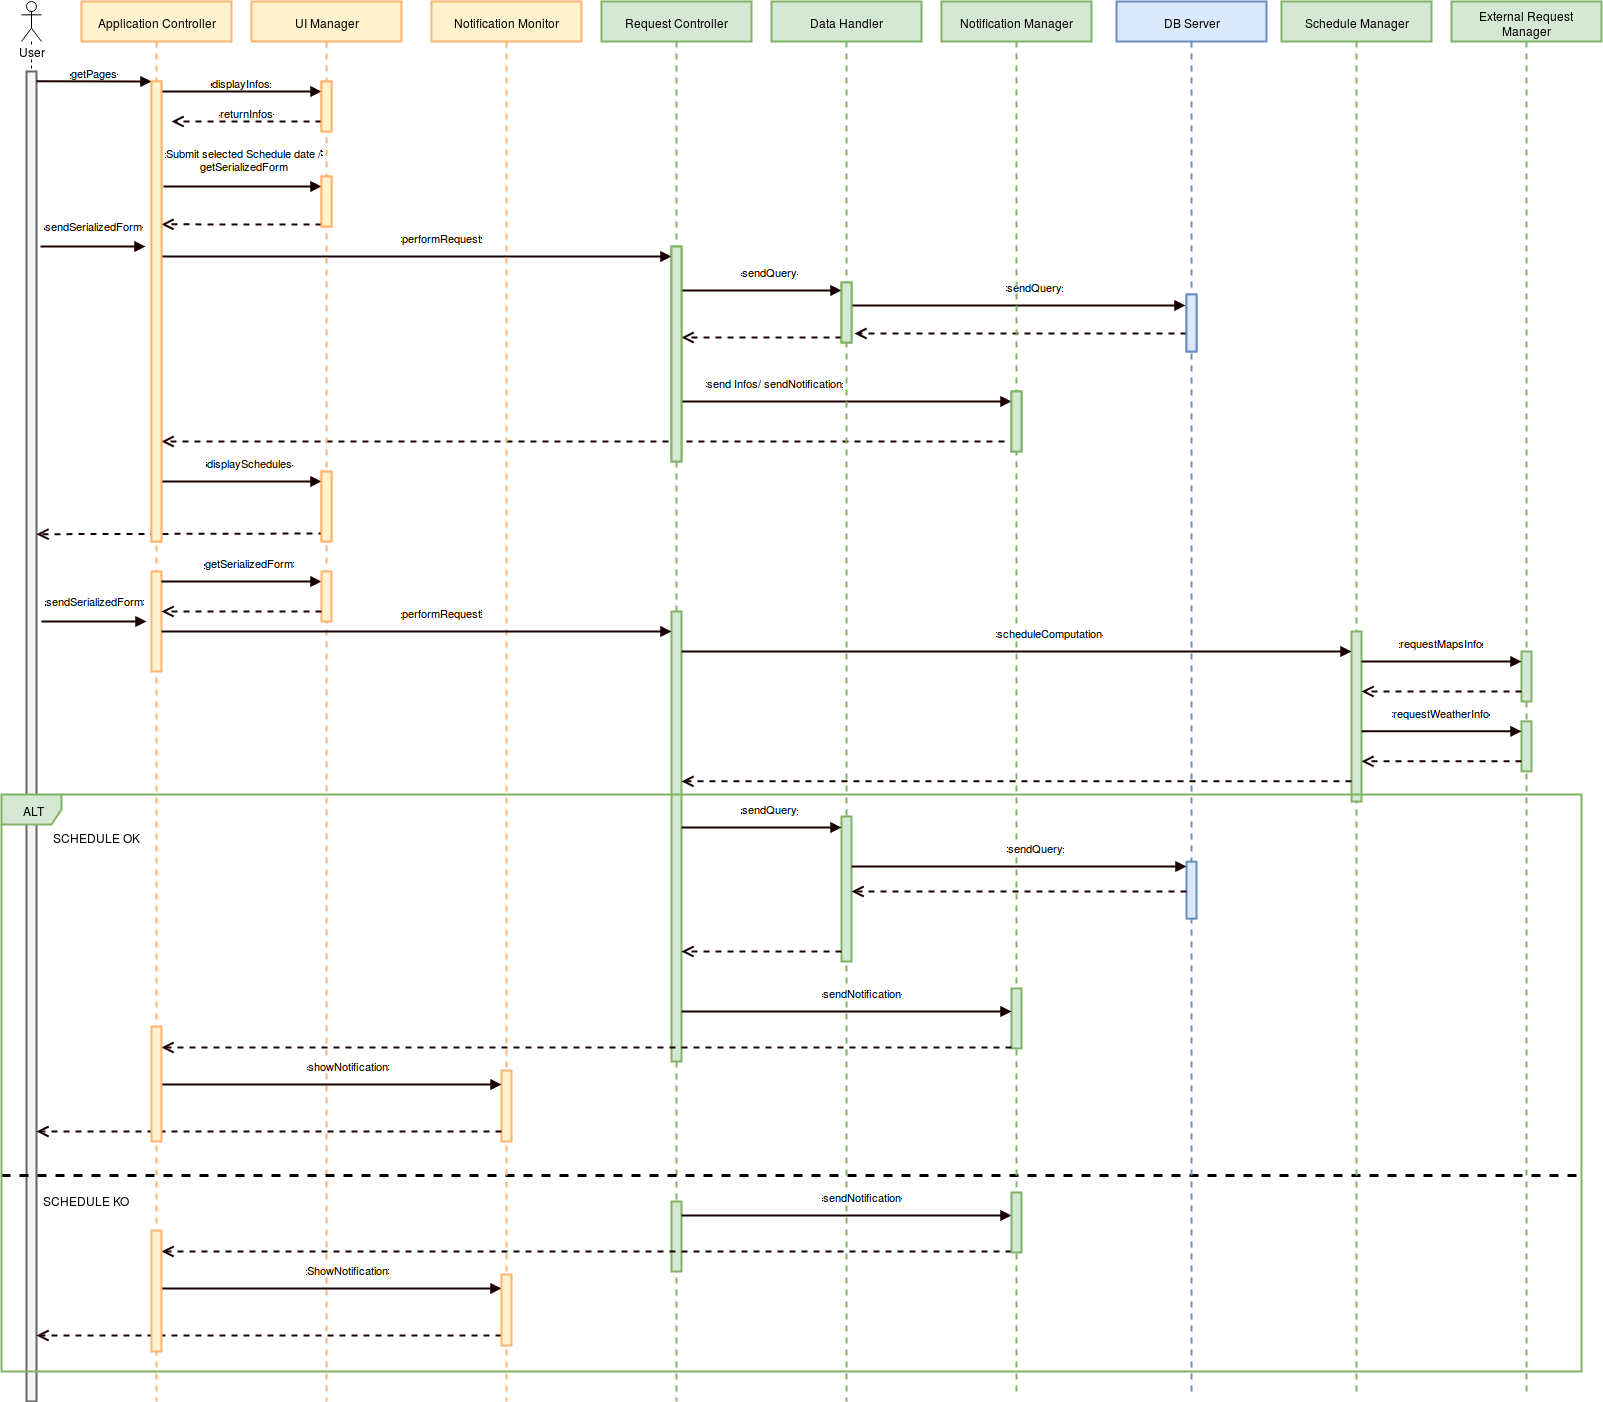
\includegraphics[width=1.1\textwidth,angle=-0]{images/Goal7}
	\caption{Sequence Diagram of updating user's schedule}
\end{figure}

As the preferences of every user are stored in the Database Server, whenever they want to change them the Data Handler's method submitQuery is called. Then the modifications are saved and updated immediatly in the DB server. 

\subsection*{Manage user's preference about time for break}

\begin{figure}[H]
	\centering
	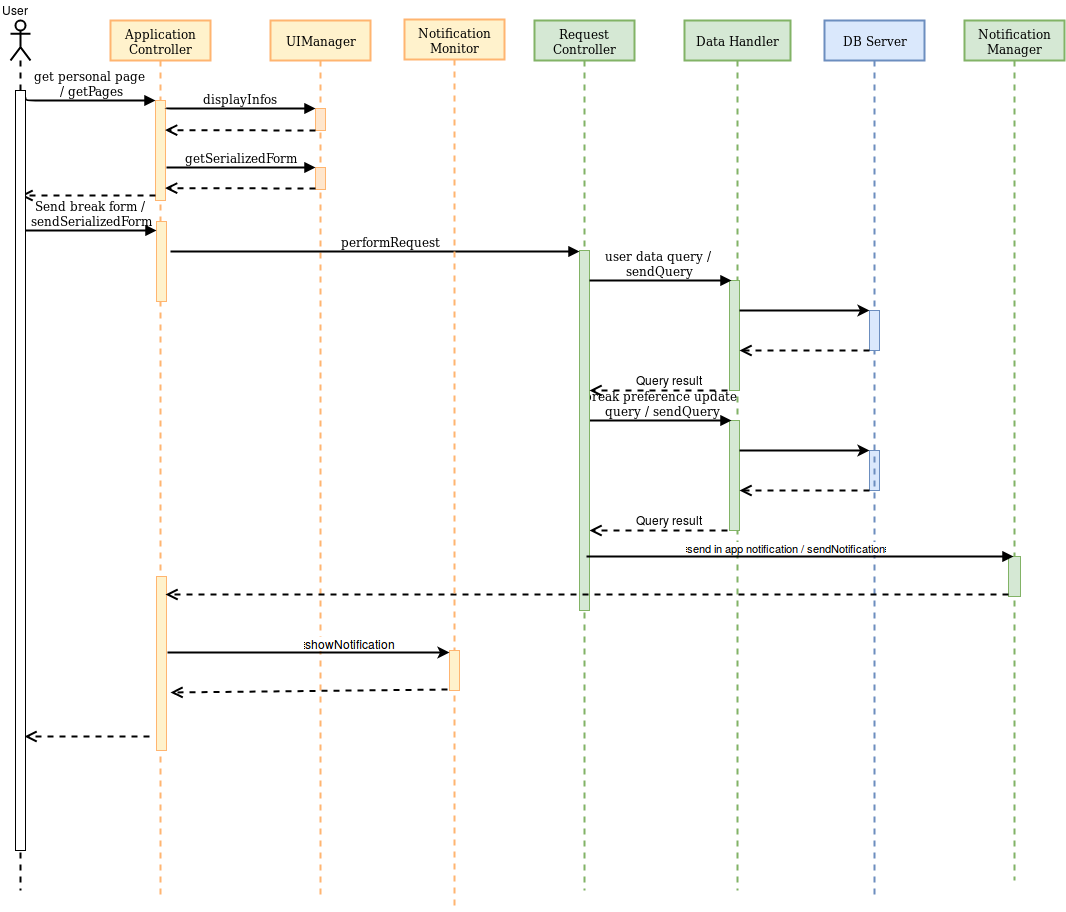
\includegraphics[width=1.1\textwidth,angle=-0]{images/Goal8}
	\caption{Sequence Diagram of managing user's preference about time for break}
\end{figure}

If a user decides to modify his break preferences, they are modified for all the upcoming schedules he decides to create. Already created schedules are not modified. 


\subsection*{User wants to see a schedule for specified day}

\begin{figure}[H]
	\centering
	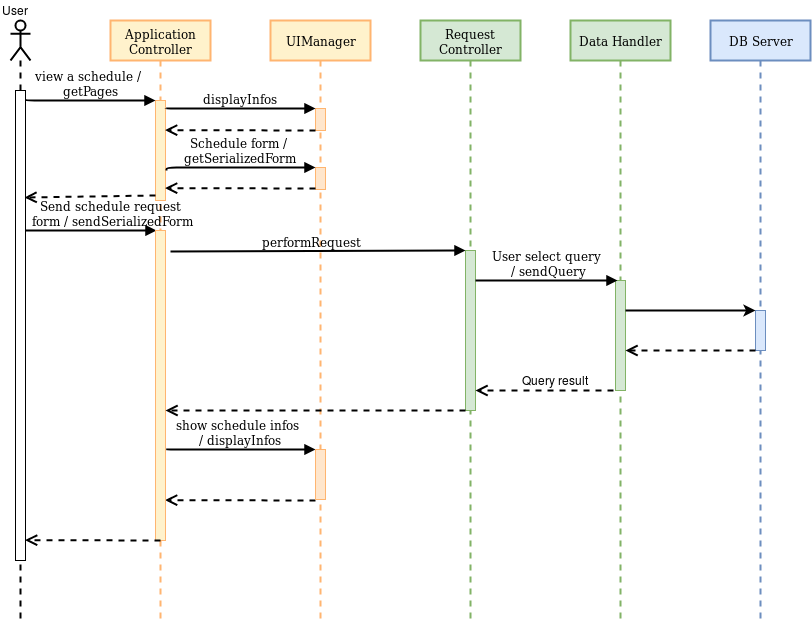
\includegraphics[width=1.1\textwidth,angle=-0]{images/Goal9}
	\caption{Sequence Diagram of a user wants to see a schedule for specified day}
\end{figure}

If a user decides to see a schedule of his, he has just to insert the data of the day and thus it will be passed to the Application Controller. Then, after a query is successfully executed passing from the Request Controller and Data Handler, the result is shown to the user by the UI Manager.

\subsection*{Other considerations}

In all the diagrams above the procedure which check the correctness of the token and the one that explain the submitQuery method to the Database server where deliberately omitted. The reason is mainly redundancy and thus they are explained in the following diagrams.\\

\subsection*{Check token procedure}

\begin{figure}[H]
	\centering
	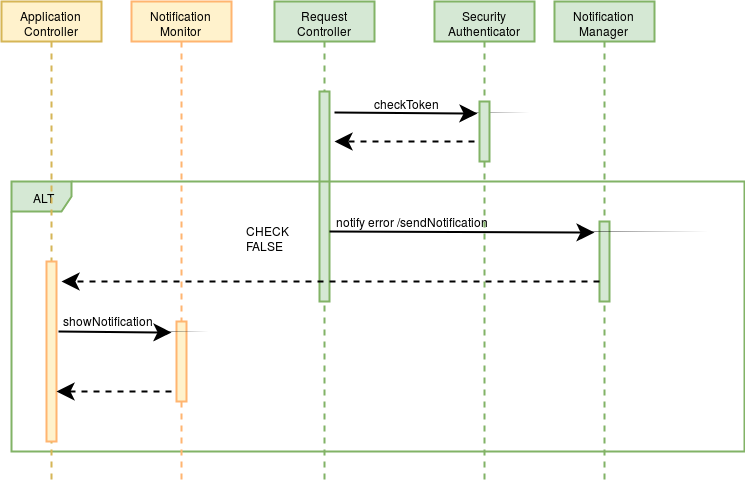
\includegraphics[width=1.1\textwidth,angle=-0]{images/checkToken}
	\caption{The procedure of checking the token}
\end{figure}

This particular procedure is called every time the user makes a request to the server. The validity of the token is then increased to permit the user an easy flow in browsing contents.

\subsection*{Query DBMS procedure}

\begin{figure}[H]
	\centering
	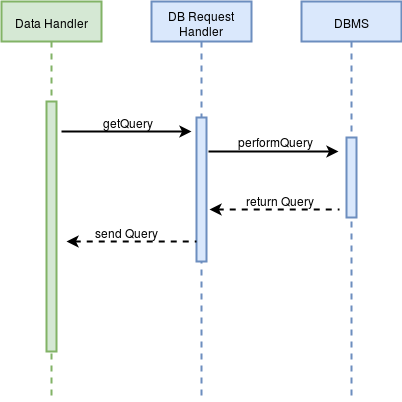
\includegraphics[width=0.7\textwidth,angle=-0]{images/QueryDBMS}
	\caption{The procedure of sending a query to the DBMS}
\end{figure}

\subsection*{Login procedure}

\begin{figure}[H]
	\centering
	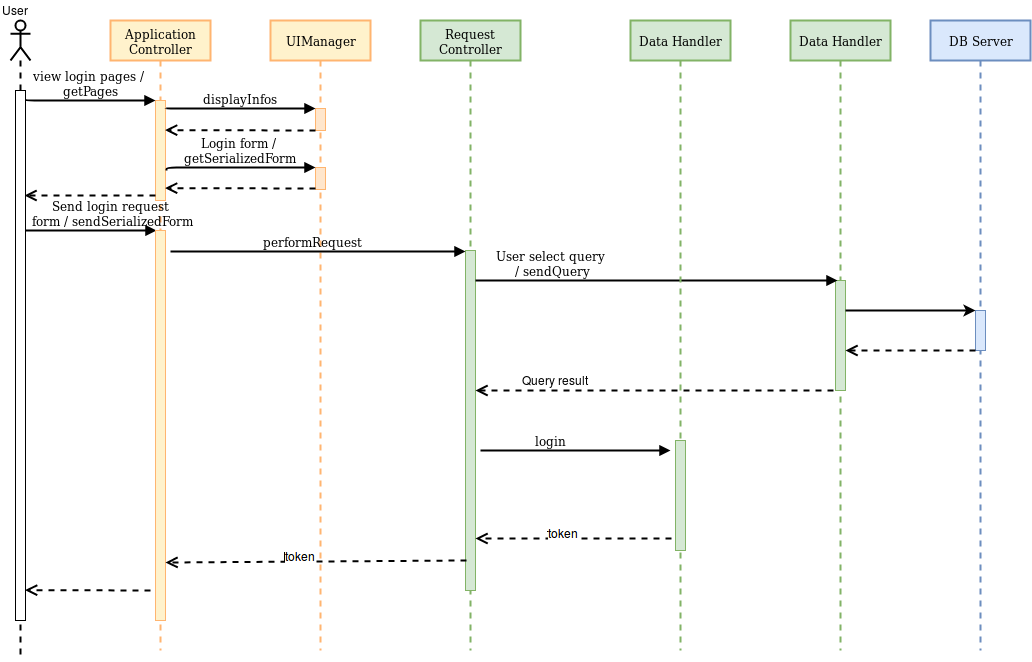
\includegraphics[width=1\textwidth,angle=-0]{images/Login}
	\caption{The procedure of logging in}
\end{figure}

\section{Component Interfaces}

This sections includes further details on the interfaces between different components of the system.

\subsection*{Component Interface of the client}

\begin{figure}[H]
	\centering
	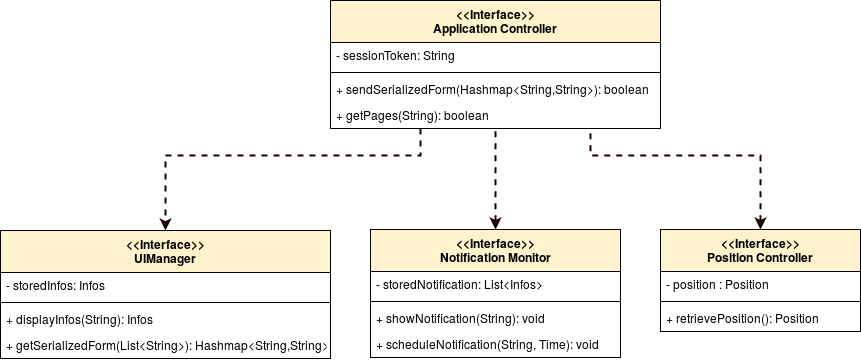
\includegraphics[width=1\textwidth]{images/ClientInterface}
	\caption{Component Interface of the client}
\end{figure}

\subsection*{Component Interface of the Application \& Web Server}


\begin{figure}[H]
	\centering
	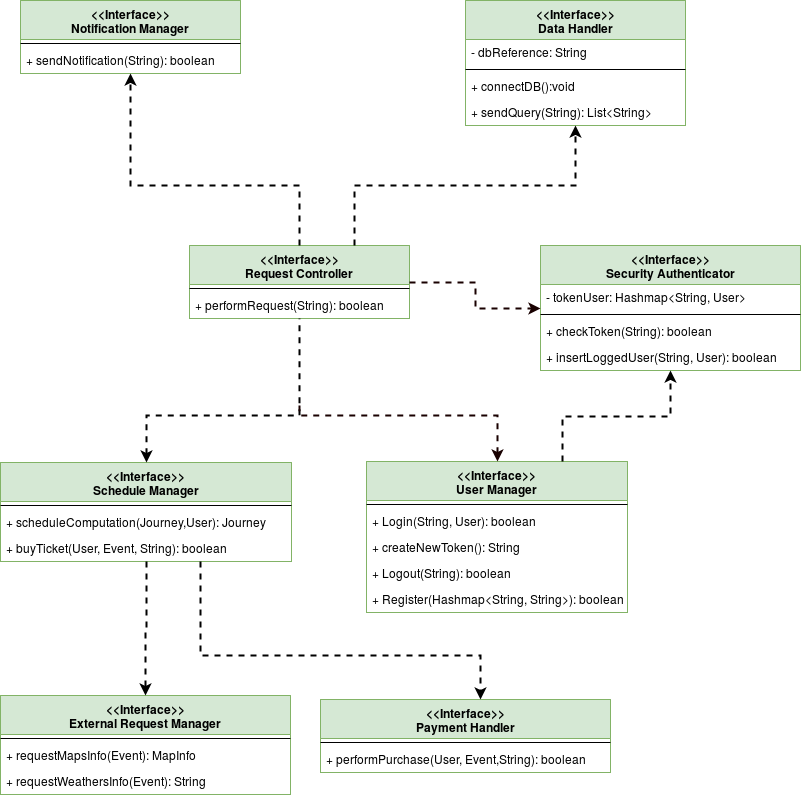
\includegraphics[width=1\textwidth]{images/ApplicationInterface}
	\caption{Component Interface of the Application \& Web Server}
\end{figure}

\subsection*{Component Interface of the Database Server}

\begin{figure}[H]
	\centering
	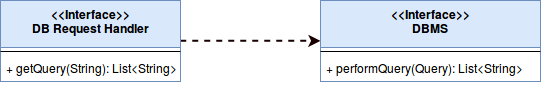
\includegraphics[width=1\textwidth]{images/DatabaseInterface}
	\caption{Component Interface of the Database Server}
\end{figure}



\section{Selected Architectural styles and patterns}

We decided to use a three-tier architecture. The client will be represented by the application installed on the device of the user or his web browser, which only contains the presentation layer. Therefore it is a so called Thin-Client.\\

On the other hand, the server is represented by a mainframe which computate all the business logic and computation to fullfill the users' requests. The reason behind this choice are the willing of keeping thin the client to improve the user experience and the reserved channel on which communicate the Application server and the Database server. As there is only this single channel, we can guarantee the confidentiality and privacy of the users. \\

Here are listed the main pattern we chose to implement:
\begin{itemize}
	\item \textbf{Model View Controller}:\\\newline
	The model role is covered by the Data center which mantains the data related to the users. The controller instead is covered by the Application \& Web Server which manage the events handling with both Model and View. Finally, the View is covered by the Client Application which displays data and informations in a way that is possibile to interact with them due to a User Interface.\\
	
	\item \textbf{Proxy}:\\\newline
	On the Application side we keep a copy of the tokens which allow the user to correctly login. In this way it is not necessary to request every time the database server in order to know if a user is currently logged in or not. Therefore we can actually even double check if a user is really connected with a random control over time.\\
	
	\item \textbf{Singleton}:\\\newline
	The Application Server's module RequestController is a Singleton, as it is istatiated only once and handle all the possibile request by different users.\\
	
\end{itemize}


\section{Other design decisions}

We decided to display on the client side a map which displays the journey the user is willing to do. In order to achive this, we decided to use the Google Maps API.\\

For the Weather Forecast instead we decided to requests informations to the OpenWeather API. In this way we can also display data about the forecast whenever the users' request them.\\

To keep stored the session of any current user, we decide to implement the login procedure based on a token-exhange and verification. Therefore is possibile to keep alive a session up to an estabilished time (for example 5 min) and refresh it whenever a correct HTTP GET is performed.\\

To ease the developement of a cross platform application, we decided to use Phonegap (https://phonegap.com/), which allows the creation of different kind of native applications starting from a WebApp. In that way it is possible to use it from iOS, Android and Windows Phone and from Desktop browsers

\chapter{Algorithm Design}

In this section we will explain the algorithms that concern the critical part of the implementation on the system.

\subsection*{Creation of a Journey/Event}

The algorithm used for the creation of a journey has to take into account every aspect of a user profile. It has to follow these steps:\\
\begin{enumerate}
	\item Consider the schedule of a chosen by user day
	\item Take informations about the Weather Forecast
	\item Take the user's preferences about the means of transport
	\item Retrieve the information about the best path to take from Google Maps API 
	\item Verify that the combination of created Event and Journey in the Schedule does not overlap with another currently existing Event or Journey
	\item Verify that there is always possibile to have an Event of type Break in the current Schedule
	\item If the previous control is satisfied we can save the update Schedule into the Database Server
	\item Else, the Application server notifies the user that something went wrong
\end{enumerate}


\subsection*{Token Creation}

This is an example of a piece of code which can be used to apply the algorithm.



\begin{lstlisting}
/**
* Generate a random string.
*/
public String nextString() {
for (int idx = 0; idx < buf.length; ++idx)
buf[idx] = symbols[random.nextInt(symbols.length)];
return new String(buf);
}

public static final String special = "!%&/=#@";

public static final String upper = "ABCDEFGHIJKLMNOPQRSTUVWXYZ";

public static final String lower = upper.toLowerCase(Locale.ROOT);

public static final String digits = "0123456789";

public static final String alphanum = upper + lower + digits;

private final Random random;

private final char[] symbols;

private final char[] buf;

public RandomString(int length, Random random, String symbols) {
if (length < 1) throw new IllegalArgumentException();
if (symbols.length() < 2) throw new IllegalArgumentException();
this.random = Objects.requireNonNull(random);
this.symbols = symbols.toCharArray();
this.buf = new char[length];
}

/**
* Create an alphanumeric string generator.
*/
public RandomString(int length, Random random) {
this(length, random, alphanum);
}

/**
* Create an alphanumeric strings from a secure generator.
*/
public RandomString(int length) {
this(length, new SecureRandom());
}

/**
* Create session identifiers.
*/
public RandomString() {
this(21);
}
\end{lstlisting}


\subsection*{User Registration}

This is an example of a piece of code which can be used to apply the algorithm.

\begin{lstlisting}
public void register(HashMap<String, String> newUser) {
try {
PreparedStatement prepared = connection
.prepareStatement("insert into User (Surname, Name, Age, Email) values (?,?,?,?)");
prepared.setString(1, newUser.get("Surname"));
prepared.setString(2, newUser.get("Name"));
prepared.setString(3, newUser.get("Age"));
prepared.setString(4, newUser.get("Email"));
prepared.executeUpdate();
} catch (SQLException e) {
e.printStackTrace();
} finally {
try {
if (connection != null)
connection.close();
} catch (SQLException e) {
e.printStackTrace();
}
}
}
\end{lstlisting}


\subsection*{Payment}

In order to perform the purchase requested by the user, the system has to follow these steps:

\begin{enumerate}
	\item Consider the mean of transport found in the event
	\item Allow the user to choose the ticket or subscription referred to the mean of transport of his choice
	\item Consider the credit card data of the user
	\item Send the purchase information to third part services like PayPal
	\item If the purchase ends well, save the receipt of the ticket and add it to the stored ticket of the user in the Database Server
	\item Else, the system notifies the user that something went wrong with the transaction
\end{enumerate}


\chapter{User Interface Design}

\subsection*{UX Diagram}

The purpose of the UX diagram is to show the different screen provided by the user interface. Moreover it points out the interactions among the screens themselves and the presence of input form and required data in a specific screen.\\

The diagram provided below follow the User Interface requirements stated in the RASD. The Web and the Mobile application implement the same  functionalities and the same screen.

\begin{figure}[H]
	\centering
	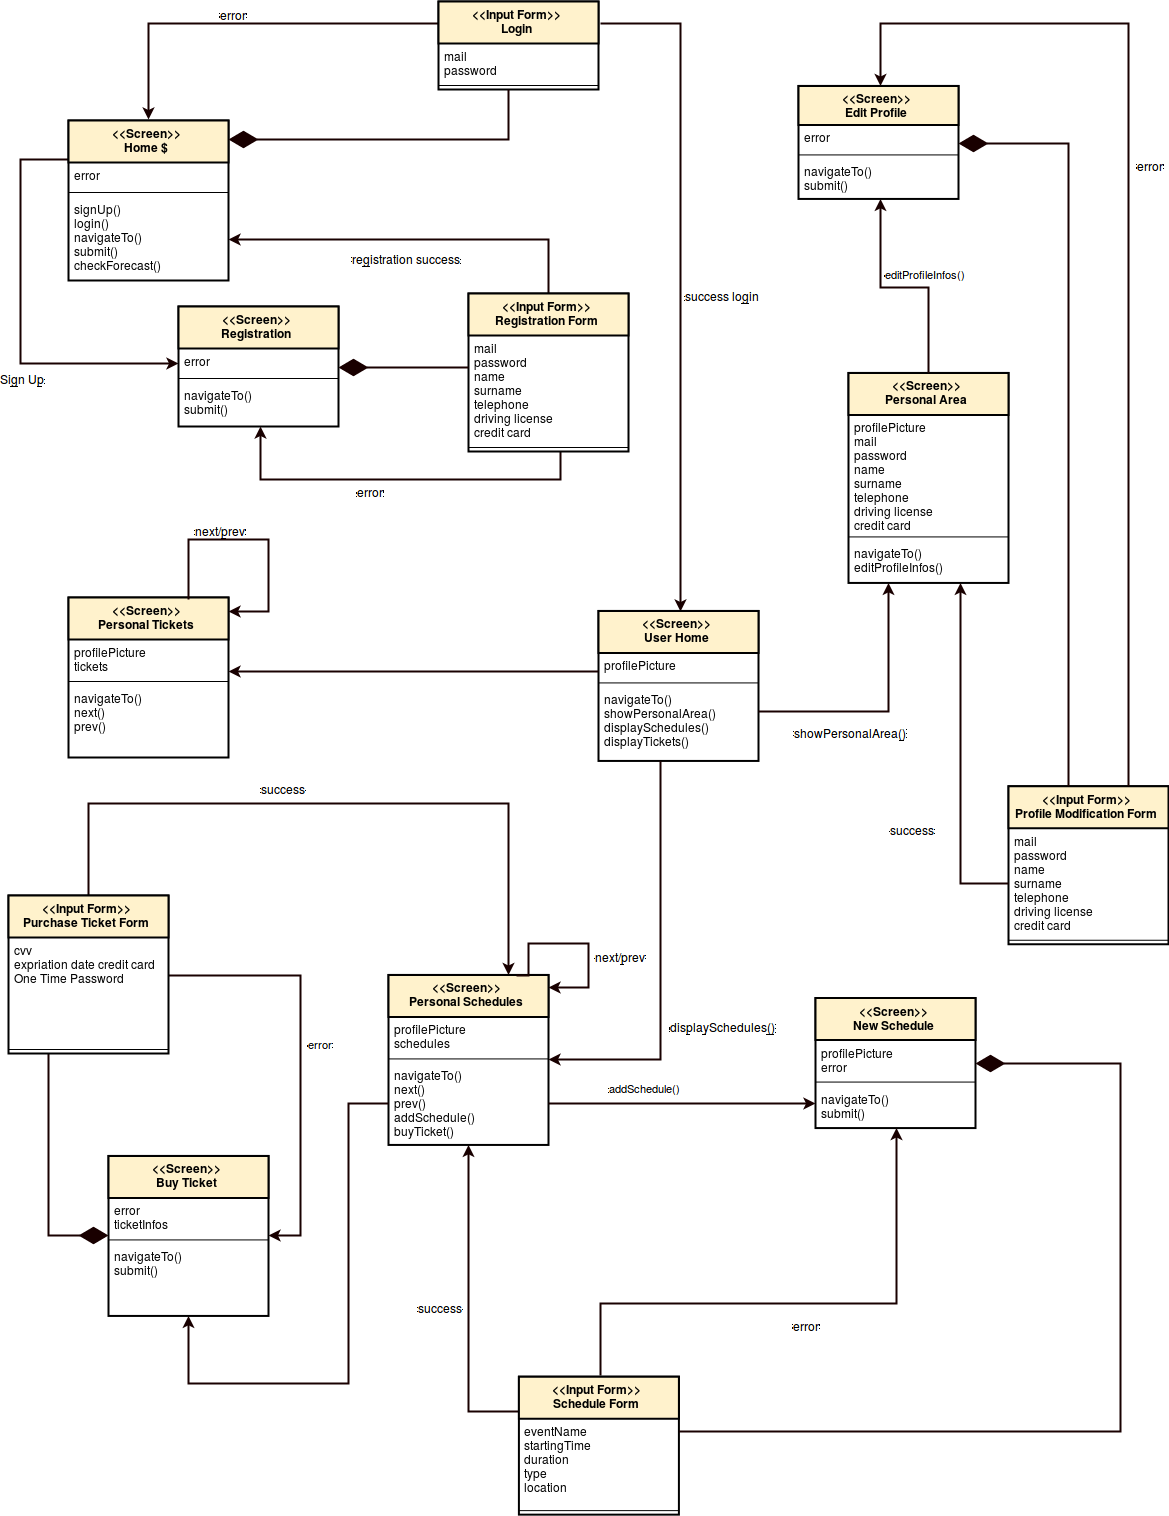
\includegraphics[width=0.9\textwidth]{images/UXDiagram2}
	\caption{Component Interface of the Database Server}
\end{figure}

\chapter{Requirements Traceability}

\chapter{Implementation,Integration and Test Plan}


\chapter{Effort Spent}


\chapter{References}

\end{document}